\subsubsection{Vzájemná poloha parametricky zadaných přímek}
\label{subsubsec:Relative_position_parametric_lines}

U parametrického vyjádření je směr přímky určen jejím směrovým
vektorem. Vzájemnou polohu dvou parametricky zadaných přímek proto
budeme určovat především porovnáním jejich směrových vektorů.

Uvažujme přímky $p$ a $q$ zadané parametricky ve tvaru
\begin{align}
    p: X &= A+t\vec{u},
    \qquad t\in\mathbb{R},
    \label{eq:Parametric_line_p_relative_position}\\
    q: X &= B+s\vec{v},
    \qquad s\in\mathbb{R},
    \label{eq:Parametric_line_q_relative_position}
\end{align}
kde $A$ a $B$ jsou zvolené body jednotlivých přímek a $\vec{u}$,
$\vec{v}$ jsou jejich nenulové směrové vektory.

Pro každou přímku používáme jiný parametr, v našem případě $t$ a $s$,
protože hodnota parametru určuje, o jaký násobek příslušného směrového
vektoru se ze zvoleného bodu posuneme. Hodnota parametru potřebná
k dosažení společného bodu z bodu $A$ proto obecně nemusí být stejná
jako hodnota parametru potřebná k dosažení téhož bodu z bodu $B$.

Vzájemnou polohu přímek určíme nejprve porovnáním jejich směrových
vektorů.

Jestliže směrové vektory $\vec{u}$ a $\vec{v}$ nejsou rovnoběžné,
tedy neexistuje číslo $k\in\mathbb{R}$, pro které by platilo
\[
    \vec{v}=k\vec{u},
\]
mají přímky různé směry. Protože obě přímky leží v jedné rovině,
protínají se právě v jednom bodě a jsou tedy různoběžné podle definice \ref{def:Intersecting_lines_plane}.

Jestliže naopak existuje číslo
$k\in\mathbb{R}\setminus\{0\}$ takové, že
\[
    \vec{v}=k\vec{u},
\]
mají přímky stejný směr. V takovém případě jsou přímky buď rovnoběžné,
nebo totožné, a proto musíme ještě ověřit, zda jeden zvolený bod jedné
přímky leží také na přímce druhé.

Pokud zvolený bod $B$ přímky $q$ neleží na přímce $p$,
nemají přímky žádný společný bod a jsou proto rovnoběžné podle definice \ref{def:Parallel_lines_plane}. 
Jestliže naopak bod $B$ na přímce $p$ leží, mají obě přímky
společný bod a zároveň stejný směr, takže jsou totožné podle definice \ref{def:Coincident_lines_plane}.

Celý rozhodovací postup můžeme shrnout následovně:
\[
\begin{array}{c|c}
\text{Podmínka}
&
\text{Vzájemná poloha přímek}
\\
\hline
\vec{u}\text{ a }\vec{v}\text{ nejsou rovnoběžné}
&
\text{přímky jsou různoběžné}
\\[1mm]
\vec{v}=k\vec{u},\ k\neq0,\ \text{a }B\notin p
&
\text{přímky jsou rovnoběžné}
\\[1mm]
\vec{v}=k\vec{u},\ k\neq0,\ \text{a }B\in p
&
\text{přímky jsou totožné}
\end{array}
\]
Rozhodovací postup můžeme také shrnout pomocí schématu na obrázku
\ref{fig:Relative_position_parametric_lines_decision}.

\begin{remark}\label{rem:Alternative_test_coincident_lines}
    Místo přímého dosazování bodu $B$ do parametrického vyjádření
    přímky $p$ můžeme určit vektor
    \[
        \overrightarrow{AB}=B-A.
    \]
    Bod $B$ leží na přímce $p$ právě tehdy, když existuje číslo
    $\lambda\in\mathbb{R}$ takové, že
    \[
        \overrightarrow{AB}=\lambda\vec{u}.
    \]
    Tato podmínka zahrnuje také případ $A=B$, pro který je
    $\lambda=0$.

    Jsou-li současně směrové vektory obou přímek rovnoběžné, jsou
    přímky totožné. Dosazování bodu do parametrického vyjádření však
    zároveň procvičuje postup potřebný při hledání průsečíku, a proto
    jej budeme v následujících příkladech používat častěji.
\end{remark}

\begin{figure}[H]
    \centering
    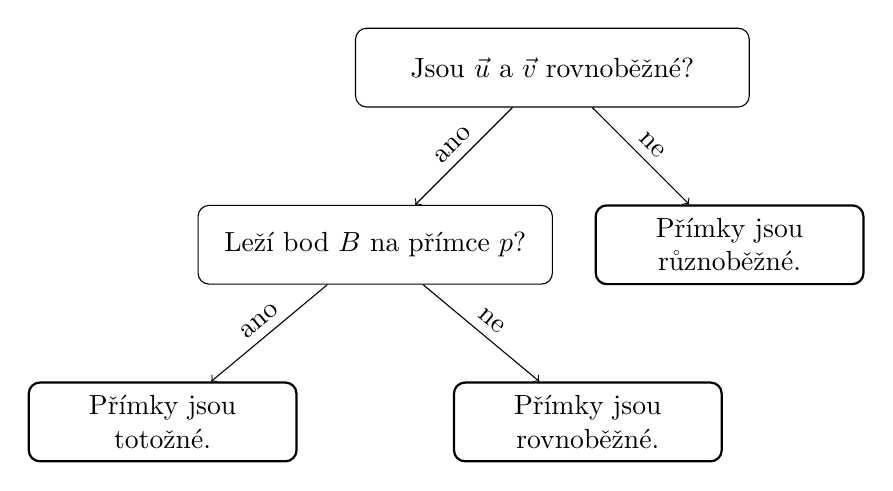
\begin{tikzpicture}[scale=0.9, every node/.style={align=center}]

        % Uzly
        \node[draw, rounded corners, minimum width=5cm, minimum height=1cm]
            (start) at (0,0)
            {Jsou $\vec{u}$ a $\vec{v}$ rovnoběžné?};

        \node[draw, rounded corners, minimum width=4.5cm, minimum height=1cm]
            (point) at (-2.5,-2.5)
            {Leží bod $B$ na přímce $p$?};

        \node[draw, rounded corners, minimum width=3.4cm, minimum height=1cm, thick]
            (intersecting) at (2.5,-2.5)
            {Přímky jsou\\různoběžné.};

        \node[draw, rounded corners, minimum width=3.4cm, minimum height=1cm, thick]
            (coincident) at (-5.5,-5)
            {Přímky jsou\\totožné.};

        \node[draw, rounded corners, minimum width=3.4cm, minimum height=1cm, thick]
            (parallel) at (0.5,-5)
            {Přímky jsou\\rovnoběžné.};

        % Šipky
        \draw[->] (start) -- (point)
            node[midway, above, sloped] {ano};

        \draw[->] (start) -- (intersecting)
            node[midway, above, sloped] {ne};

        \draw[->] (point) -- (coincident)
            node[midway, above, sloped] {ano};

        \draw[->] (point) -- (parallel)
            node[midway, above, sloped] {ne};

    \end{tikzpicture}
    \caption{Postup při určování vzájemné polohy parametricky zadaných přímek v rovině.}
    \label{fig:Relative_position_parametric_lines_decision}
\end{figure}

\paragraph{Rovnoběžné přímky}

Jak již bylo řečeno, jsou-li směrové vektory dvou přímek navzájem rovnoběžné, nemůžeme pouze
z této skutečnosti rozhodnout, zda jsou přímky rovnoběžné, nebo totožné.
Musíme ještě ověřit, zda jeden zvolený bod jedné přímky leží také na
druhé přímce.

\begin{example}\label{exa:Parallel_parametric_lines}
    Určete vzájemnou polohu přímek $p$ a $q$ zadaných bodem
    a směrovým vektorem:
    \[
        p:\ A[-1;3],\qquad \vec{u}=(-1;2),
    \]
    \[
        q:\ B[1;1],\qquad \vec{v}=(2;-4).
    \]

    Nejprve zjistíme, zda jsou směrové vektory $\vec{u}$ a $\vec{v}$
    navzájem rovnoběžné. Hledáme tedy číslo $k\in\mathbb{R}$, pro které
    platí
    \[
        \vec{v}=k\vec{u}.
    \]

    Po dosazení souřadnic dostáváme
    \[
        (2;-4)=k(-1;2).
    \]
    Z jednotlivých souřadnic vyplývá
    \begin{align*}
        2 &= -k \Rightarrow  k=-2,\\
        -4 &= 2k \Rightarrow k=-2.
    \end{align*}

    Z obou souřadnic vyšla stejná hodnota $k=-2$, a proto jsou směrové
    vektory rovnoběžné. Přímky $p$ a $q$ jsou tedy buď rovnoběžné,
    nebo totožné.

    Nyní ověříme, zda bod $A[-1;3]$ leží na přímce $q$. Parametrické
    vyjádření přímky $q$ je
    \begin{align*}
        q: x &= 1+2s,\\
           y &= 1-4s;
           \quad s\in\mathbb{R}.
    \end{align*}

    Dosadíme souřadnice bodu $A[-1;3]$:
    \begin{align*}
        -1 &= 1+2s,\\
        3 &= 1-4s.
    \end{align*}

    Z první rovnice získáme
    \begin{align*}
        -1 &= 1+2s,\\
        -2 &= 2s,\\
        s &= -1.
    \end{align*}
    Z druhé rovnice však vychází
    \begin{align*}
        3 &= 1-4s,\\
        2 &= -4s,\\
        s &= -\tfrac{1}{2}.
    \end{align*}

    Z rovnic vyšly různé hodnoty parametru, takže bod $A$ na přímce
    $q$ neleží. Přímky mají rovnoběžné směrové vektory, ale nemají
    společný bod, a proto jsou rovnoběžné:
    \[
        p\parallel q.
    \]
\end{example}

\paragraph{Různoběžné přímky a jejich průsečík}

Jestliže směrové vektory dvou přímek nejsou navzájem rovnoběžné, jsou
přímky v rovině různoběžné a mají právě jeden společný bod. Tento bod
nazýváme \textbf{průsečíkem přímek}.

Průsečík musí současně ležet na obou přímkách, a jeho souřadnice proto
musí vyhovovat parametrickým rovnicím přímky $p$ i přímky $q$. Při
hledání průsečíku tedy položíme odpovídající souřadnice obou přímek
sobě rovny a vyřešíme vzniklou soustavu rovnic.

\begin{remark}\label{rem:Different_parameters_parametric_lines}
    Při porovnávání dvou parametricky vyjádřených přímek musíme pro
    každou přímku použít jiný parametr. Zápisy
    \[
        p:\ X=A+t\vec{u}
        \qquad\text{a}\qquad
        q:\ X=B+s\vec{v}
    \]
    proto používají parametry $t$ a $s$.

    Stejný bod může být totiž na první přímce získán například pro
    $t=1$, zatímco na druhé přímce může témuž bodu odpovídat hodnota
    $s=-1$. Použití stejného parametru v obou přímkách by znamenalo
    neoprávněný předpoklad, že se k průsečíku z obou zvolených bodů
    dostaneme pomocí stejného násobku rozdílných směrových vektorů.
\end{remark}

\begin{example}\label{exa:Intersecting_parametric_lines}
    Určete vzájemnou polohu přímek
    \[
        \begin{aligned}
            p:\quad x &= -1+3t,\\
                     y &= 1+t;
                     \quad t\in\mathbb{R}
        \end{aligned}
        \qquad\text{a}\qquad
        \begin{aligned}
            q:\quad x &= 1-s,\\
                     y &= -2s;
                     \quad s\in\mathbb{R}.
        \end{aligned}
    \]
    Jsou-li přímky různoběžné, určete jejich průsečík.

    Směrové vektory přímek jsou
    \[
        \vec{u}=(3;1),
        \qquad
        \vec{v}=(-1;-2).
    \]

    Nejprve ověříme, zda existuje číslo $k$, pro které platí
    \[
        \vec{v}=k\vec{u}.
    \]
    Z první souřadnice dostáváme
    \[
        -1=3k
        \qquad\Rightarrow\qquad
        k=-\frac13,
    \]
    zatímco z druhé souřadnice získáme
    \[
        -2=k.
    \]

    Hodnoty čísla $k$ se neshodují, takže směrové vektory nejsou
    rovnoběžné. Přímky $p$ a $q$ jsou proto různoběžné a mají právě
    jeden průsečík.

    Souřadnice průsečíku musí vyhovovat oběma parametrickým vyjádřením.
    Položíme proto odpovídající souřadnice sobě rovny:
    \begin{align*}
        p_x &= q_x,\\
        p_y &= q_y,
    \end{align*}
    což po dosazení parametrických rovnic přímek $p$ a $q$ dává soustavu
    \begin{align*}
        -1+3t &= 1-s,\\
        1+t &= -2s.
    \end{align*}

    Po úpravě získáme soustavu
    \begin{align*}
        3t+s &= 2,\\
        t+2s &= -1.
    \end{align*}

    Z první rovnice vyjádříme parametr $s$:
    \[
        s=2-3t.
    \]
    Dosadíme do druhé rovnice, abychom získali hodnotu parametru $t$:
    \begin{align*}
        t+2(2-3t) &= -1,\\
        t+4-6t &= -1,\\
        -5t &= -5,\\
        t &= 1.
    \end{align*}

    Hodnotu parametru $s$ dopočítáme zpětným dosazením do vztahu pro $s$:
    \[
        s=2-3\cdot1=-1.
    \]

    Souřadnice průsečíku nyní vypočítáme dosazením parametru $t=1$
    do parametrického vyjádření přímky $p$:
    \begin{align*}
        x &= -1+3\cdot1=2,\\
        y &= 1+1=2.
    \end{align*}

    Průsečíkem přímek je tedy bod
    \[
        P[2;2].
    \]

    Výsledek můžeme ověřit také dosazením hodnoty $s=-1$ do přímky $q$:
    \begin{align*}
        x &= 1-(-1)=2,\\
        y &= -2\cdot(-1)=2.
    \end{align*}

    Řešením soustavy rovnic pro parametry je dvojice
    \[
        (t;s)=(1;-1).
    \]
    Po dosazení jedné z těchto hodnot do odpovídajícího parametrického
    vyjádření jsme získali společný bod
    \[
        P[2;2].
    \]

    Průsečíkem přímek $p$ a $q$ je proto bod $P[2;2]$, což zapisujeme
    \[
        p\cap q=\{P[2;2]\}.
    \]
    
\end{example}

\begin{remark}\label{rem:Parameters_are_not_intersection_coordinates}
    Hodnoty parametrů $t$ a $s$ nejsou souřadnicemi průsečíku.
    Parametry pouze určují, jakým násobkem směrového vektoru se musíme
    posunout ze zvoleného bodu příslušné přímky. Souřadnice průsečíku
    získáme až následným dosazením vypočítané hodnoty parametru do
    parametrického vyjádření jedné z přímek.
\end{remark}

\paragraph{Totožné přímky}

Jsou-li směrové vektory dvou přímek rovnoběžné a zároveň jeden zvolený
bod první přímky leží na druhé přímce, obsahují obě přímky tentýž bod
a mají stejný směr. V takovém případě mají všechny body společné a jsou
totožné.

\begin{example}\label{exa:Coincident_parametric_lines}
    Určete vzájemnou polohu přímek
    \[
        \begin{aligned}
            p:\quad x &= -2 + 2t,\\
                    y &= 1 - t;
                    \quad t\in\mathbb{R}
        \end{aligned}
        \qquad\text{a}\qquad
        \begin{aligned}
            q:\quad x &= 4 - 4s,\\
                    y &= -2 + 2s;
                    \quad s\in\mathbb{R}.
        \end{aligned}
    \]
    Z parametrických rovnic vyčteme zvolené body a směrové vektory:
    \[
        A[-2;1],
        \qquad
        \vec{u}=(2;-1),
    \]
    \[
        B[4;-2],
        \qquad
        \vec{v}=(-4;2).
    \]

    Směrové vektory jsou rovnoběžné, protože
    \[
        \vec{v}=-2\vec{u}.
    \]

    Přímky jsou proto buď rovnoběžné, nebo totožné. 
    Ověříme, zda bod $A[-2;1]$ leží na přímce $q$. Dosadíme jeho souřadnice:
    \begin{align*}
        -2 &= 4-4s,\\
        1 &= -2+2s.
    \end{align*}

    Z první rovnice získáme
    \[
        s=\frac32,
    \]
    a z druhé rovnice rovněž
    \[
        s=\frac32.
    \]

    Bod $A$ tedy leží na přímce $q$. Přímky mají rovnoběžné směrové
    vektory a společný bod, a proto jsou totožné:
    \[
        p=q.
    \]

    Totožnost můžeme ověřit také řešením soustavy rovnic pro společné
    body:
    \begin{align*}
        -2+2t &= 4-4s,\\
        1-t &= -2+2s.
    \end{align*}

    Po úpravě první rovnice dostáváme
    \[
        t+2s=3,
    \]
    zatímco úpravou druhé rovnice získáme tutéž podmínku
    \[
        t+2s=3.
    \]

    Obě rovnice soustavy jsou tedy ekvivalentní, takže soustava má nekonečně mnoho řešení. 
    Každému bodu přímky odpovídá dvojice parametrů $t$ a $s$, která splňuje vztah
    \[
        t+2s=3.
    \]
    Protože má soustava nekonečně mnoho řešení, 
    mají přímky nekonečně mnoho společných bodů. Jejich průnikem je tedy celá přímka:
    \[
        p\cap q=p=q.
    \]
\end{example}

\paragraph{Kolmé přímky}

Kolmost je zvláštním případem různoběžnosti. Dvě parametricky zadané
přímky jsou kolmé právě tehdy, když jsou kolmé jejich směrové vektory.

Pro přímky se směrovými vektory $\vec{u}$ a $\vec{v}$ tedy platí
\[
    p\perp q
    \quad\Longleftrightarrow\quad
    \vec{u}\cdot\vec{v}=0.
\]

Protože jsou směrové vektory nenulové, nemohou být v tomto případě
rovnoběžné. Kolmé přímky se tedy v rovině protínají právě v jednom
bodě.

Určování průsečíku dvou parametricky vyjádřených přímek můžeme využít
také v geometrických úlohách. Typickým příkladem je výpočet souřadnic
paty výšky v trojúhelníku, protože pata výšky je průsečíkem přímky
obsahující jednu stranu trojúhelníku a přímky, která prochází protějším
vrcholem a je k této straně kolmá.

\begin{example}\label{exa:Foot_of_altitude_parametric_lines}
    Určete souřadnice paty výšky $v_c$ v trojúhelníku $ABC$, jehož
    vrcholy jsou
    \[
        A[-2;-1],\qquad B[6;-5],\qquad C[3;4].
    \]

    Výška $v_c$ je vedena z vrcholu $C$ kolmo ke straně $AB$.
    Její pata, kterou označíme $P_C$, proto leží současně na přímce
    obsahující stranu $AB$ i na výšce $v_c$. Bod $P_C$ tedy nalezneme
    jako průsečík těchto dvou přímek.

    Nejprve určíme směrový vektor přímky obsahující stranu $AB$:
    \[
        \overrightarrow{AB}
        =
        (6-(-2);-5-(-1))
        =
        (8;-4).
    \]

    Směrový vektor můžeme nahradit jeho jednodušším nenulovým násobkem:
    \[
        \vec{u}_{AB}=(2;-1).
    \]

    Přímka $p_{AB}$ procházející bodem $A[-2;-1]$ má tedy parametrické
    vyjádření
    \begin{align*}
        p_{AB}: x &= -2+2t,\\
                y &= -1-t;
                \quad t\in\mathbb{R}.
    \end{align*}

    Směrový vektor výšky $v_c$ musí být kolmý ke směrovému vektoru
    $\vec{u}_{AB}=(2;-1)$. Můžeme proto zvolit například vektor
    \[
        \vec{u}_{v_c}=(1;2),
    \]
    protože
    \[
        (2;-1)\cdot(1;2)=2-2=0.
    \]

    Výška $v_c$ prochází vrcholem $C[3;4]$, a proto má parametrické
    vyjádření
    \begin{align*}
        v_c: x &= 3+s,\\
             y &= 4+2s;
             \quad s\in\mathbb{R}.
    \end{align*}

    Pata výšky $P_C$ leží na obou přímkách, a proto musí její souřadnice
    vyhovovat oběma parametrickým vyjádřením. Položíme tedy odpovídající
    souřadnice sobě rovny:
    \begin{align*}
        -2+2t &= 3+s,\\
        -1-t &= 4+2s.
    \end{align*}

    Po úpravě získáme soustavu
    \begin{align*}
        2t-s &= 5,\\
        t+2s &= -5.
    \end{align*}

    Z první rovnice vyjádříme parametr $s$:
    \[
        s=2t-5.
    \]

    Dosadíme jej do druhé rovnice:
    \begin{align*}
        t+2(2t-5) &= -5,\\
        t+4t-10 &= -5,\\
        5t &= 5,\\
        t &= 1.
    \end{align*}

    Hodnotu parametru $s$ dopočítáme zpětným dosazením:
    \[
        s=2\cdot1-5=-3.
    \]

    Souřadnice paty výšky získáme například dosazením hodnoty $t=1$
    do parametrického vyjádření přímky $p_{AB}$:
    \begin{align*}
        x &= -2+2\cdot1=0,\\
        y &= -1-1=-2.
    \end{align*}

    Pata výšky $v_c$ má tedy souřadnice
    \[
        P_C[0;-2].
    \]

    Výsledek můžeme ověřit také dosazením hodnoty $s=-3$ do
    parametrického vyjádření výšky:
    \begin{align*}
        x &= 3+(-3)=0,\\
        y &= 4+2\cdot(-3)=-2.
    \end{align*}

    Obě parametrická vyjádření určují stejný bod, a proto je hledanou
    patou výšky skutečně bod
    \[
        P_C[0;-2].
    \]
\end{example}